\chapter{Introduction}
Quantum Field Theory (QFT) represents the modern language to describe particle physics. It combines consistently quantum principles and special relativity using the concept of spacetime fields. The dynamics of the fields is based on symmetries in Nature. In particular, the interactions between particles are described in gauge theories which show a redundancy under local group transformations.\\

The best description of the fundamental laws which govern the elementary particles and their interactions is given by the Standard Model (SM). Developed in the 1970s, this is a QFT based on the symmetry group $SU(3)_C\cross SU(2)_L \cross U(1)_Y$. Quantum cromodynamics (QCD) describes the strong interactions between gluons and quarks and it is related to the exact symmetry of the theory under $SU(3)_C$ transformations. The subgroup $SU(2)_L \cross U(1)_Y$ defines the electroweak interactions and this symmetry is spontaneously broken in $U(1)_{em}$ by the Brout-Englert-Higgs mechanism.\\

High energy predictions are generally tested in colliders. The SM has a huge success in predicting the experimental datas: it is the most successful physical model ever. One of the main reasons of the construction of CERN's Large Hadron Collider (LHC) was the research of the last undetected particle of the SM. This is the excitement of the Higgs field responsible for the spontaneous electroweak symmetry breaking and, consequently, for the mass of all the SM particles. On 4th July 2012, the collaboration of ATLAS and CMS experiments at LHC announced the discovery of a new scalar particle \cite{ATLAS:2012yve, CMS:2012qbp}. One of the goals of the current particle phenomenology is the study of the properties of the Higgs boson.\\
Despite its success, the SM cannot describe completely the Nature. For example, the SM does not foresee the neutrino oscillations or the presence of dark matter and dark energy which represent the most abundant components in the Universe.\\
In order to investigate the effects from a physics beyond the Standard Model (BSM), it is necessary a good knowledge of the SM background (mainly coming from QCD) by computing the predictions at every increasing precision level.\\

At LHC proton-proton collisions at $14\,TeV$ are produced. The use of massive hadrons helps to achieve high energies, but the signals are more complicated than the events in lepton colliders. Indeed, protons are composite particles and there are two different processes which occur during the collision. By introducing a factorization scale, we can separate long range effects concerned with the hadron structure from short range contributions. Using Feynman's parton model, we can describe the cross section of a deep inelastic scattering between two protons with momenta $P_1$ and $P_2$,
\begin{align*}
	\sigma(pp\rightarrow X)=\sum_{f_1,f_2=\{g,u,d,\dots,\bar u, \bar d, \dots\}}  \int_0^1 \dd x_1 \int_0^1 \dd x_2 \, f_{f_1}(x_1,\mu_F^2) f_{f_2}(x_2,\mu_F^2) \hat \sigma\left(f_1 f_2 \rightarrow X; x_1 P_1, x_2 P_2, \mu_R^2, \mu_F^2\right).
\end{align*}
The result is the incoherent sum of contributions from the elementary scattering of two partons $f_1$ and $f_2$ which carry the momenta $x_1 P_1$ and $x_2 P_2$. We introduced the factorization scale $\mu_F$ and the energy scale $\mu_R$ in which we operate the renormalization.\\
The Parton Distribution Functions (PDFs) $f_{f_i}(x_i)$ are non-perturbative objects which give the probability of finding the parton $f_i$ (gluon or quark) in the hadron. They are extracted from datas combining the information from different experiments. In particular a fundamental contribution came from DESY's HERA, a lepton-proton collider (1992-2007). The PDFs depends on the factorization scale and the evo\-lution from low to high scale can be computed theoretically using the renormalization group equation, the Dokshitzer-Gribov-Lipatov-Altarelli-Parisi (DGLAP) equation \cite{Altarelli:1977zs}. Recent progress in PDFs are the full next-to-next-leading-order (NNLO) evolution and the computation of new PDFs (photon, leptons, W and Z boson).\\
\begin{figure}[H]
\begin{center}
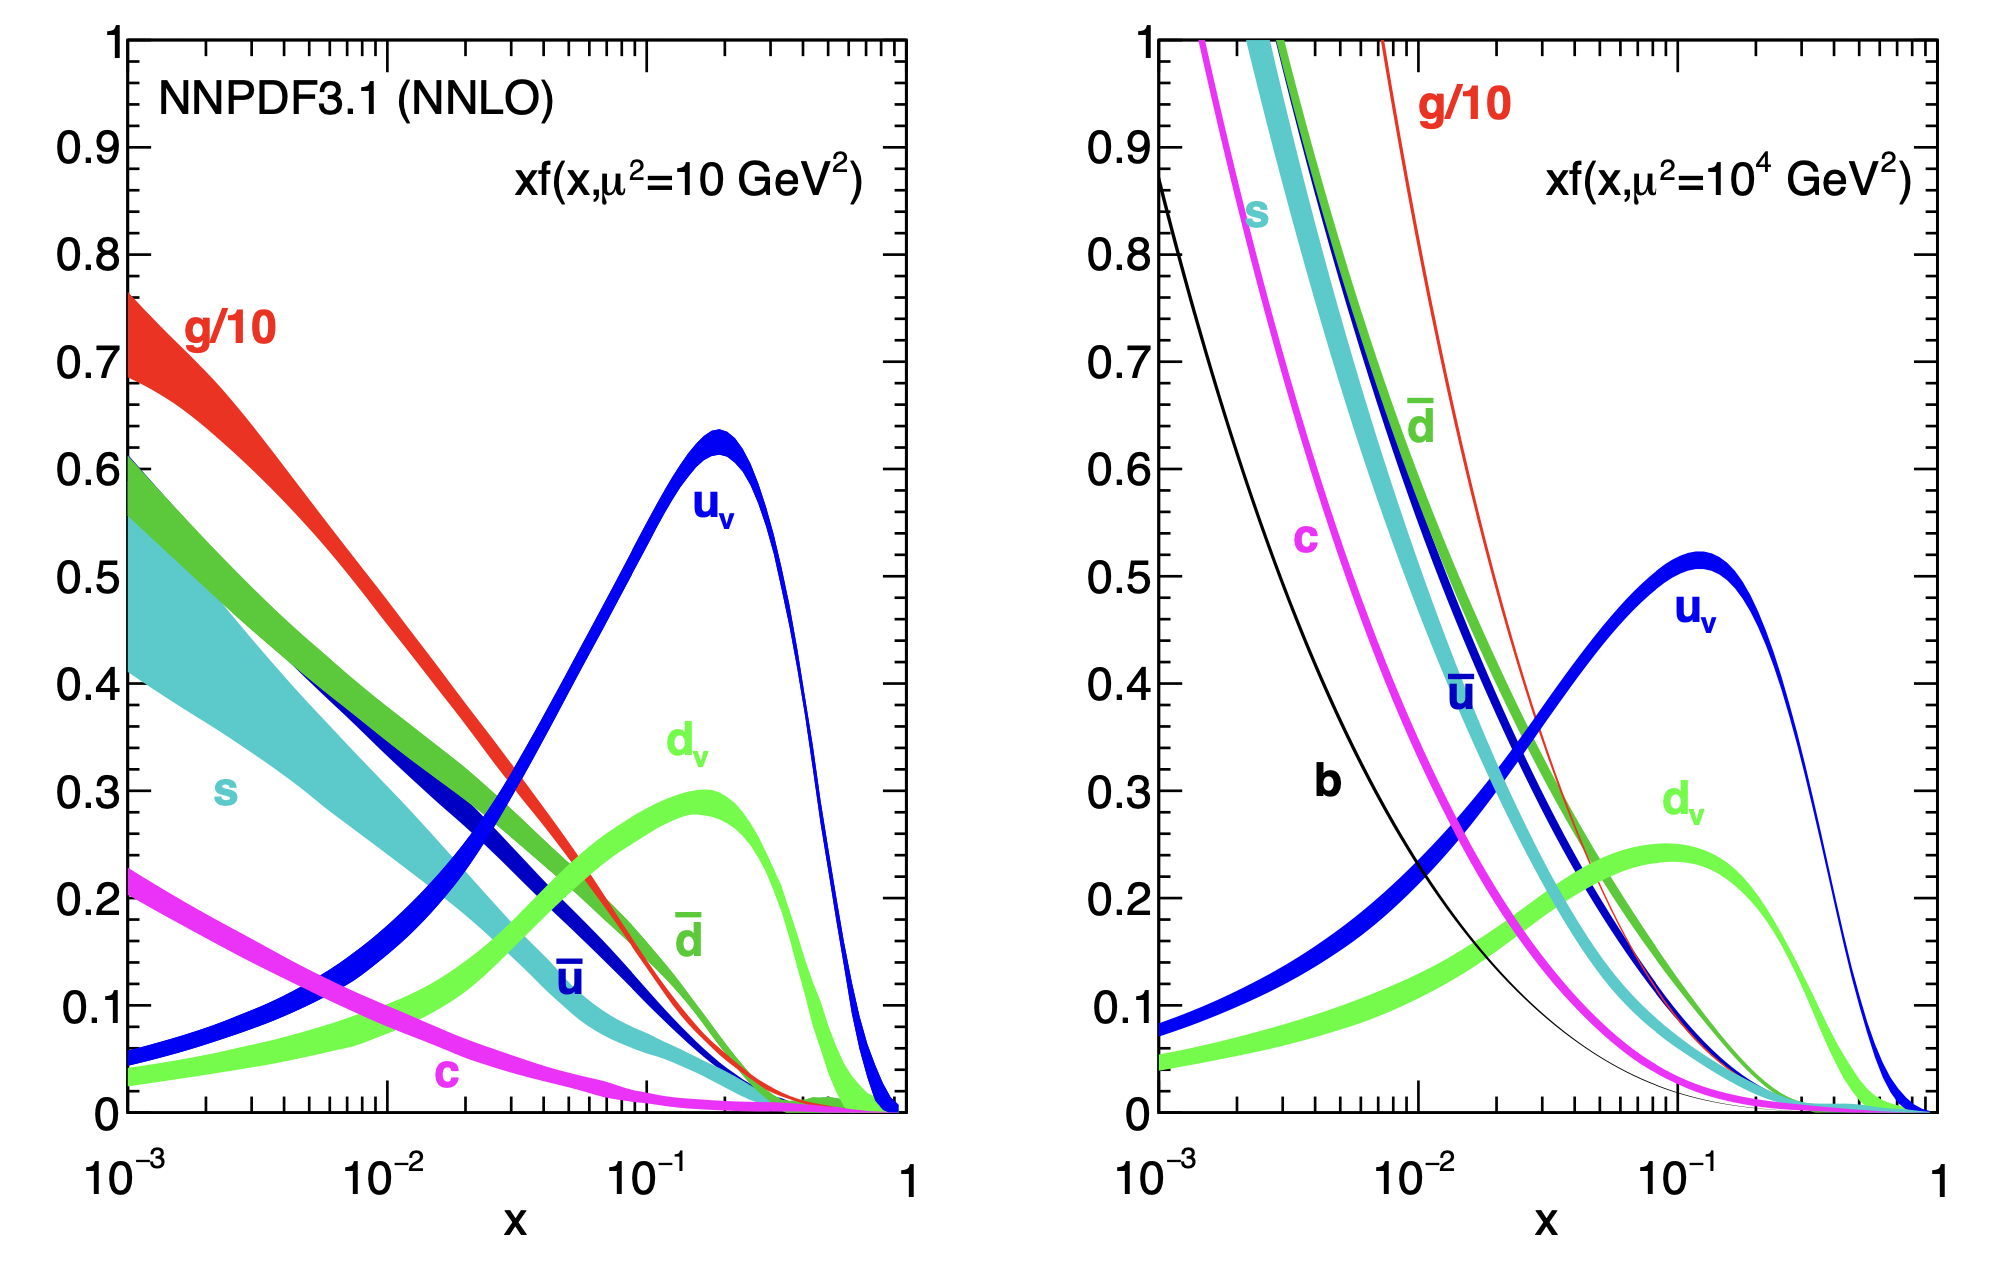
\includegraphics[width=0.95\textwidth]{protonPDFs}
\caption{Gluon and quark PDFs for the proton obtained in NNLO NNPDF3.1 analysis \cite{Ball_2017} at scale $\mu_F^2=10\,GeV^2$ (left) and $\mu_F^2=10^4\,GeV^2$ (right).}
\end{center}
\end{figure}

Gluon and sea quark distributions grow at small $x$, in particular gluon dominates at small longitudinal momentum fraction. Differently to what typically observed in elementary scattering processes, cross sections in hadron colliders increase with the energy. Indeed, we need smaller $x$ in order to produce the same mass state and the cross section grows due to the behavior of PDFs at small $x$.\\
For example, the Higgs production ($m_H\simeq 125\,GeV$) in a collision at $14\,TeV$ is dominated by gluons because, from kinematical considerations, the needed momentum fraction is $x\simeq 10^{-2}$. For this reason, the interaction between two gluons through a quark loop in order to produce the Higgs boson is the main channel for the production of this scalar particle. This process is known as the \textit{gluon gluon fusion} (ggF).\\

After the hard collision, the QCD products undergo a \textit{jet fragmentation process} due to the confinement property of strong interactions. Indeed, the signals in the detector are hadrons with high transverse momentum forming jets.\\
Firstly, soft radiations are emitted from final states of the hard scattering process. The probability of no gluon emissions above some transverse momentum is encoded in the Sudakov form factor which is used to generate the gluon distribution by Monte Carlo (MC) methods. In order to complete a real description of an event simulation, we have to include the hadronisation. Only a color-neutral collection of partons can be observed as an isolate system, then the MC event generators should implement this process. Currently, the most used implementations are based on string \cite{Andersson:1983ia} or cluster \cite{Chahal:2022rid} hadronisation models.\\
\newpage

The parton level cross section $\hat \sigma$ describes the hard scattering and is related to the fundamental interactions between elementary fields. This prediction can be calculated perturbatively because of the asymptotic freedom of QCD. The cross section is related to the squared matrix element,
\begin{align*}
	\hat \sigma(f_1 f_2 \rightarrow X)=\frac{\mathcal{S}}{2 \hat s} \int \dd \Pi_n \, \delta^{(4)}\left(\text{total momentum}\right) \left| \mathcal{A}(f_1 f_2 \rightarrow X)\right|^2,
\end{align*}
where $\mathcal{S}$ is a symmetry factor related to the identical particles in the final state and $\hat s$ is the center of mass energy for the parton process. We have to integrate over the Lorentz invariant phase space measure for the $n$ outgoing particles which are in the set $X$ and have momenta $q_i$,
$$
	\int \dd \Pi_n = \prod_i \int \frac{\dd^3 q_i}{2E_i (2\pi)^3}.
$$
The scattering amplitude $\mathcal{A}(f_1 f_2 \rightarrow X)$ is the fundamental ingredient which describes the interaction between the elementary particles. It represents a bridge between the QFT model and the phenomenology. In order to compute the amplitude, according to the traditional approach we should start from the Lagrangian, extract the Feynman rules for propagators and interaction vertices, compute all the allowed Feynman diagrams and sum together. The number of diagrams quickly increases with the number of external asymptotic states and with the number of loops. Furthermore, in squaring the amplitude, we have to compute quantum interferences between Feynman diagrams and this increases the complexity of the calculation.\\
Firstly, we can fix the polarization of the asymptotic states, namely the helicity for massless particles. The complexity is reduced because different helicity configurations do not interfere in the squared amplitude. Then we have to compute only a sum of squared helicity amplitudes,
\begin{align*}
	\left| \mathcal{A}(a+\dots \rightarrow b+\dots)\right|^2= \sum_{h_a, h_b, \dots} | \mathcal{A}(a^{h_a} +\dots \rightarrow b^{h_b} +\dots)|^2.
\end{align*}
Surprising structures of helicity amplitudes were found indeed they are simpler than the expectation from a sum of many Feynman diagrams. The complexity of helicity amplitudes depends on how much they violate the helicity conservation. The simplest structures are observed in the subset of not-vanishing helicity amplitudes which describe the processes with the maximal helicity violation, known as MHV amplitudes. In 1986, Parke and Taylor \cite{Parke:1986gb} predicted the structure of MHV amplitudes in gauge theories for an arbitrary number of gluons in terms of rational functions of kinematic invariants.\\
Moreover, the unitarity of the theory shows a connection between the discontinuity of loop amplitudes and on-shell amplitudes with lower levels of precision.
Modern techniques have been developed in order to compute one-loop and two-loop amplitudes using generalisations of the unitarity approach. One of the main reasons of the complexity of traditional computations is related to gauge redundancy. Feynman diagrams are not individually invariants differently to the result, then strong cancellations arise only when we sum together all the contributions. On-shell methods use tree-level amplitude as the building blocks for predictions of higher precision level, then they fully exploit the gauge invariance of the theory.\\

The cross section for the Higgs boson ggF production is currently known at next-to-next-to-next leading order ($\text{N}^3\text{LO}$) in QCD corrections \cite{Anastasiou_2015}. NNLO is the current level of precision of QCD corrections for the Higgs production in association with a jet \cite{Boughezal_2015}. The complexity of the computation increases with additional jets indeed for the Higgs production with two jets only NLO QCD corrections was computed \cite{an_Deurzen_2013}. These predictions are calculated in the Higgs Effective Field Theory (HEFT) in which the dominant contribution to ggF, the top-quark loop, is integrated out in the limit of infinite top mass $m_t$. This method reduces the number of loops we have to compute by one, but it is necessary a good control of the validity of this approximation. NLO predictions with the full top-mass effects are computed for the Higgs+jet production \cite{Harlander_2012, Jones_2018}. HEFT seems to works because the Higgs mass is below $2m_t$, which is the case of phenomenological interest. However, the quality of the heavy-top limit is limited by effects on Higgs' transverse momentum $p_{t,H}$: HEFT is a good approximation for $p_{t,H}<200 GeV$ as one can see in the Figure [\ref{fig:pt}]. 
\begin{figure}[H]
\begin{center}
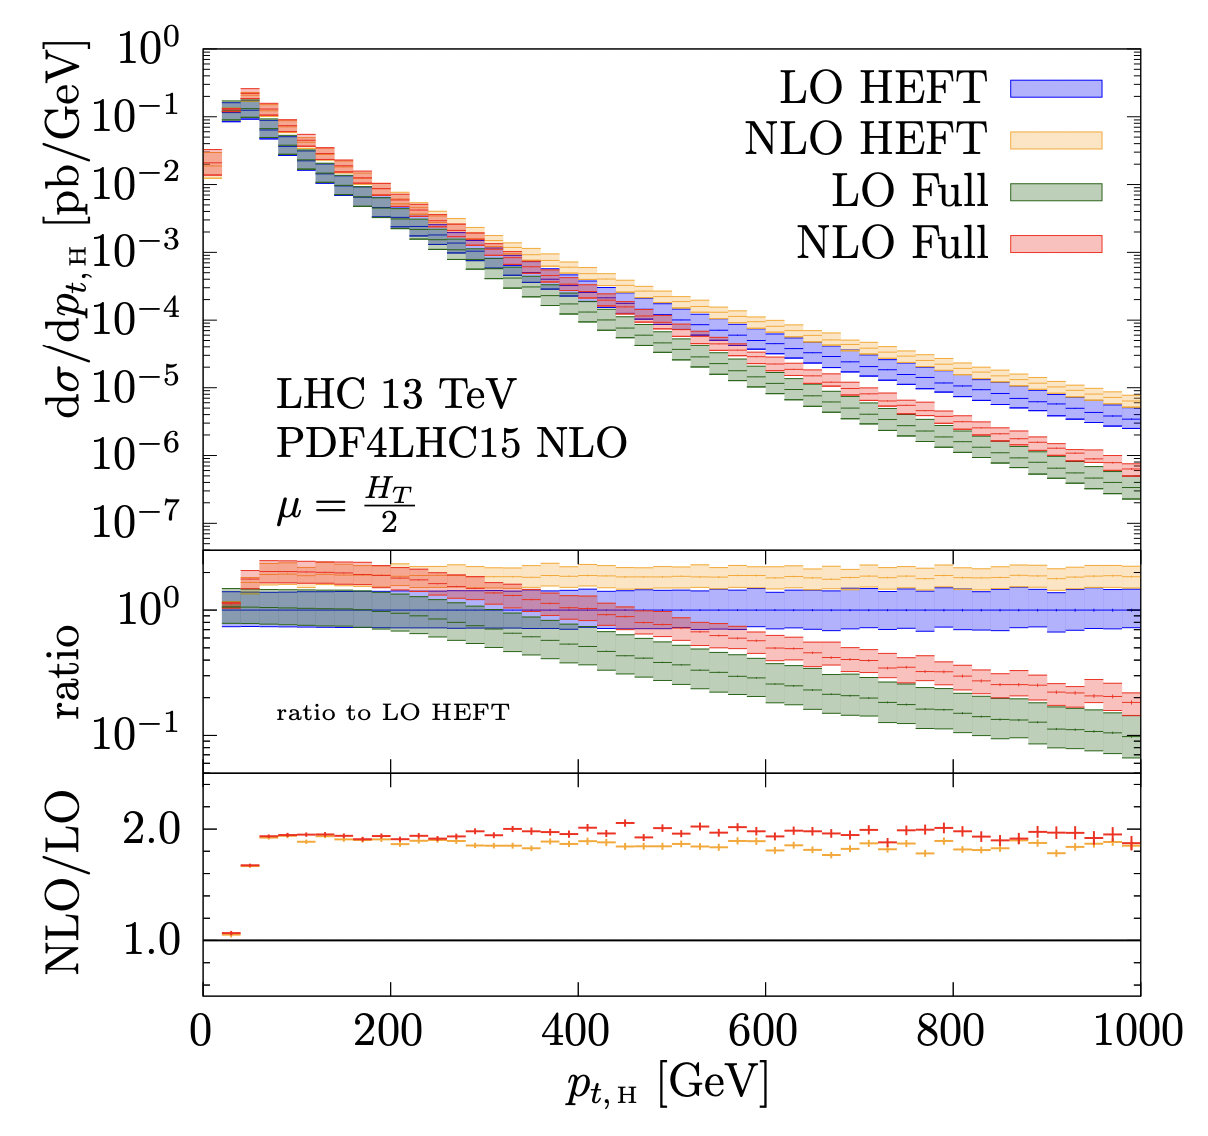
\includegraphics[width=0.6\textwidth]{Higgspt}
\caption{Higgs boson transverse momentum spectrum in QCD LO and QCD NLO for the Higgs+jet production. Comparison between the HEFT predictions and the results with the full top-mass dependence. For $p_t<200 GeV$ we observe a good agreement between the two approaches. \cite{Jones_2018}}
\label{fig:pt}
\end{center}
\end{figure}

In order to improve the level of precision for Higgs plus two jets, QCD two-loop virtual corrections represent a fundamental ingredient in NNLO computations. The desired two-loop amplitude $\mathcal{A}(gg\rightarrow Hgg)$ is not currently known in the HEFT. In an interesting version of the effective field theory, we can decompose the Higgs into two scalar fields $\phi$ and $\phi^\dagger$ whose interactions with gluons are endowed with self-dual properties. On-shell $\phi$ plus gluon amplitudes show simpler structures, in particular the MHV tree amplitude has the same form of Parke-Taylor formula.\\

In Chapter [\ref{onshellamp}], we review the spinor helicity formalism and some on-shell methods at tree and loop level. Led by the analogy between $\phi$+gluon and pure QCD MHV amplitudes, Chapter [\ref{secYM}] is devoted to the study of known one-loop and two-loop amplitudes in the all-plus sector of Yang-Mills. This represents an interesting background to learn the generalised unitarity methods in four dimensions and cuts in generic dimensions.\\
In the next chapter, we introduce the self-dual Higgs theory and we will review some useful tree and one-loop amplitudes which describe the coupling between the self-dual Higgs ($\phi$) and gluons. Also for the study of these amplitudes we implement some on-shell techniques discussed in Chapter [\ref{onshellamp}].\\
In Chapter [\ref{ch:cuts}], we compute the discontinuities of the two-loop amplitude which involves the self-dual Higgs field ($\phi$) and four gluons with positive helicity. The cut-constructible part of this amplitude represents the original result of this project.\\
In the first appendix we report the notations and the expressions for the one-loop scalar integrals.\\
In App. [\ref{appC}], we describe the computation of quadruple cuts, a generalised unitarity method applied to investigate the box contributions in the amplitude.\\
App. [\ref{phi+3g}] is devoted to the computation of the discontinuities for the amplitude at lower multiplicity considering the self-dual Higgs and only three gluons. These could be useful as a preliminary introduction for the cut computations before studying the more challenging case in Chapter [\ref{ch:cuts}]. The computation is necessary in order to check the collinear limit of the $\phi$ plus four gluon amplitude.
